% # 5.2 原子操作和原子类型

原子操作是个不可分割的操作。系统的所有线程中,不可能观察到原子操作完成了一半。如果读取对象的加载操作是原子的,那么这个对象的所有修改操作也是原子的,所以加载操作得到的值要么是对象的初始值,要么是某次修改操作存入的值。

另一方面,非原子操作可能会被另一个线程观察到只完成一半。如果这个操作是一个存储操作,那么其他线程看到的值,可能既不是存储前的值,也不是存储的值。如果非原子操作是一个读取操作,可能先取到对象的一部分,然后值被另一个线程修改,然后它再取到剩余的部分,所以它取到的既不是第一个值,也不是第二个值。这就构成了数据竞争(见5.1节),出现未定义行为。

\mySubsubsection{5.2.1}{标准原子类型}

标准原子类型定义在头文件\texttt{<atomic>}中。这些类型的操作都是原子的,语言定义中只有这些类型的操作是原子的,也可以用互斥锁来模拟原子操作。标准原子类型的实现可能是这样的:它们(几乎)都有一个\texttt{is\_lock\_free()}成员函数,这个函数可以让用户查询某原子类型的操作是直接用的原子指令(\texttt{x.is\_lock\_free()}返回\texttt{true}),还是内部用了一个锁结构(\texttt{x.is\_lock\_free()}返回\texttt{false})。

原子操作可以替代互斥量,来完成同步操作。如果操作内部使用互斥量实现,那么不可能有性能的提升。所以要对原子操作进行实现,最好使用不基于互斥量的实现。

标准库提供了一组宏,在编译时对各种整型原子操作是否无锁进行判别。C++17中,所有原子类型有一个static constexpr成员变量,如果相应硬件上的原子类型X是无锁类型,那么X::is\_always\_lock\_free将返回true。例如:给定目标硬件平台\texttt{std::atomic<int>}无锁,那么\texttt{std::atomic<int>::is\_always\_lock\_free}将会返回true。不过\texttt{std::atomic<uintmax\_t>}因为这是一个运行时属性,所以\texttt{std::atomic<uintmax\_t>::is\_always\_lock\_free}在该平台编译时可能为\texttt{false}。

宏都有\texttt{ATOMIC\_BOOL\_LOCK\_FREE},\texttt{ATOMIC\_CHAR\_LOCK\_FREE},\texttt{ATOMIC\_CHAR16\_T\_LOCK\_FREE},\texttt{ATOMIC\_CHAR32\_T\_LOCK\_FREE},\texttt{ATOMIC\_WCHAR\_T\_LOCK\_FREE},\texttt{ATOMIC\_SHORT\_LOCK\_FREE},\texttt{ATOMIC\_INT\_LOCK\_FREE},\texttt{ATOMIC\_LONG\_LOCK\_FREE},\texttt{ATOMIC\_LLONG\_LOCK\_FREE}和\texttt{ATOMIC\_POINTER\_LOCK\_FREE}。它们指定了内置原子类型的无锁状态和无符号对应类型(LLONG对应long long,POINTER对应所有指针类型)。如果原子类型不是无锁结构,那么值为0。如果原子类型是无锁结构,那么值为2。如果原子类型的无锁状态在运行时才能确定,那么值为1。

只有\texttt{std::atomic\_flag}类型不提供\texttt{is\_lock\_free()}。该类型是一个简单的布尔标志,并且在这种类型上的操作都是无锁的。当有一个简单无锁的布尔标志时,可以使用该类型实现一个简单的锁,并且可以实现其他基础原子类型。对\texttt{std::atomic\_flag}明确初始化后,做查询和设置(使用test\_and\_set()成员函数),或清除(使用clear()成员函数)都很容易:无赋值,无拷贝,没有测试和清除,没有任何多余操作。

剩下的原子类型都可以通过特化\texttt{std::atomic<>}得到,并且拥有更多的功能,但不可能都是无锁的(如之前解释的那样)。主流平台上,原子变量是无锁的内置类型(例如\texttt{std::atomic<int>}和\texttt{std::atomic<void*>})。后面会看到,每个特化接口所反映出的类型特点,比如:位操作(如:\&=)就没有为普通指针所定义,所以它就不能为原子指针所定义。

除了直接使用\texttt{std::atomic<>}模板外,也可以使用在表5.1中所示的原子类型集。由于历史原因,原子类型已经添加入C++标准中,这些备选类型名可能参考相应的\texttt{std::atomic<>}特化类型,或是特化类型。同一程序中混合使用备选名与\texttt{std::atomic<>}特化类名,会使代码的可移植性大打折扣。

表5.1 标准原子类型的备选名和与其相关的\texttt{std::atomic<>}特化类

% | 原子类型 | 相关特化类 |
% | ------------ | -------------- |
% | atomic_bool | std::atomic&lt;bool> |
% | atomic_char | std::atomic&lt;char> |
% | atomic_schar | std::atomic&lt;signed char> |
% | atomic_uchar | std::atomic&lt;unsigned char> |
% | atomic_int | std::atomic&lt;int> |
% | atomic_uint | std::atomic&lt;unsigned> |
% | atomic_short | std::atomic&lt;short> |
% | atomic_ushort | std::atomic&lt;unsigned short> |
% | atomic_long | std::atomic&lt;long> |
% | atomic_ulong | std::atomic&lt;unsigned long> |
% | atomic_llong | std::atomic&lt;long long> |
% | atomic_ullong | std::atomic&lt;unsigned long long> |
% | atomic_char16_t | std::atomic&lt;char16_t> |
% | atomic_char32_t | std::atomic&lt;char32_t> |
% | atomic_wchar_t | std::atomic&lt;wchar_t> |

C++标准库不仅提供基本原子类型,还定义了与原子类型对应的非原子类型,就如同标准库中的\texttt{std::size\_t}。如表5.2所示这些类型:

表5.2 标准原子类型定义(typedefs)和对应的内置类型定义(typedefs)

% | 原子类型定义 | 标准库中相关类型定义 |
% | ------------ | -------------- |
% | atomic_int_least8_t | int_least8_t |
% | atomic_uint_least8_t | uint_least8_t |
% | atomic_int_least16_t | int_least16_t |
% | atomic_uint_least16_t | uint_least16_t |
% | atomic_int_least32_t | int_least32_t |
% | atomic_uint_least32_t | uint_least32_t |
% | atomic_int_least64_t | int_least64_t |
% | atomic_uint_least64_t | uint_least64_t |
% | atomic_int_fast8_t | int_fast8_t |
% | atomic_uint_fast8_t | uint_fast8_t |
% | atomic_int_fast16_t | int_fast16_t |
% | atomic_uint_fast16_t | uint_fast16_t |
% | atomic_int_fast32_t | int_fast32_t |
% | atomic_uint_fast32_t | uint_fast32_t |
% | atomic_int_fast64_t | int_fast64_t |
% | atomic_uint_fast64_t | uint_fast64_t |
% | atomic_intptr_t | intptr_t |
% | atomic_uintptr_t | uintptr_t |
% | atomic_size_t | size_t |
% | atomic_ptrdiff_t | ptrdiff_t |
% | atomic_intmax_t | intmax_t |
% | atomic_uintmax_t | uintmax_t |

好多种类型!不过,它们有一个相当简单的模式。对于标准类型进行typedef T,相关的原子类型就在原来的类型名前加上atomic\_的前缀:atomic\_T。除了singed类型的缩写是s,unsigned的缩写是u,和long long的缩写是llong之外,这种方式也同样适用于内置类型。对于\texttt{std::atomic<T>}模板,使用相应的T类型去特化模板的方式,要好于使用别名的方式。

通常,标准原子类型不能进行拷贝和赋值,它们没有拷贝构造函数和拷贝赋值操作符。但是,可以隐式转化成对应的内置类型,所以这些类型依旧支持赋值,可以使用\texttt{load()}和\texttt{store()}、\texttt{exchange()}、\texttt{compare\_exchange\_weak()}和\texttt{compare\_exchange\_strong()}。它们都支持复合赋值符:+=, -=, *=, |= 等等。并且使用整型和指针的特化类型还支持++和--操作。当然,这些操作也有功能相同的成员函数所对应:fetch\_add(), fetch\_or()等等。赋值操作和成员函数的返回值,要么是存储值(赋值操作),要么是操作值(命名函数),这就能避免赋值操作符返回引用。

\texttt{std::atomic<>}类模板不仅仅是一套可特化的类型,作为原发模板也可以使用自定义类型创建对应的原子变量。因为是通用类模板,操作限制为\texttt{load()},\texttt{store()}(赋值和转换为用户类型),\texttt{exchange()},\texttt{compare\_exchange\_weak()}和\texttt{compare\_exchange\_strong()}。

每种函数类型的操作都有一个内存序参数,这个参数可以用来指定存储的顺序。5.3节中,会对存储顺序选项进行详述。现在,只需要知道操作分为三类:

1. \textit{Store}操作,可选如下内存序:\texttt{memory\_order\_relaxed}, \texttt{memory\_order\_release}, \texttt{memory\_order\_seq\_cst}。
2. \textit{Load}操作,可选如下内存序:\texttt{memory\_order\_relaxed}, \texttt{memory\_order\_consume}, \texttt{memory\_order\_acquire}, \texttt{memory\_order\_seq\_cst}。
3. \textit{Read-modify-write}(读-改-写)操作,可选如下内存序:\texttt{memory\_order\_relaxed}, \texttt{memory\_order\_consume}, \texttt{memory\_order\_acquire}, \texttt{memory\_order\_release}, \texttt{memory\_order\_acq\_rel}, \texttt{memory\_order\_seq\_cst}。

现在,让我们来看一下每个标准原子类型的操作,从\texttt{std::atomic\_flag}开始吧。

\mySubsubsection{5.2.2}{std::atomic\_flag}

\texttt{std::atomic\_flag}是最简单的原子类型,这个类型的对象可以在两个状态间切换:设置和清除。就是这么简单,只作为构建块存在。我从未期待这个类型被使用,除非在十分特别的情况下。正因如此,它将作为讨论其他原子类型的起点,因为它会展示原子类型可使用的策略。

\texttt{std::atomic\_flag}类型的对象必须被ATOMIC\_FLAG\_INIT初始化。初始化标志位是“清除”状态。这里没得选择,这个标志总是初始化为“清除”:

\begin{cpp}
std::atomic_flag f = ATOMIC_FLAG_INIT;
\end{cpp}

这适用于任何对象的声明,是唯一需要以如此特殊的方式初始化的原子类型,但也是唯一保证无锁的类型。首次使用时,需要初始化。如果\texttt{std::atomic\_flag}是静态存储的,那么就的保证其是静态初始化的,也就意味着没有初始化顺序问题。

当标志对象已初始化,只能做三件事情:销毁,清除或设置(查询之前的值)。这些操作对应的函数分别是:clear()成员函数和test\_and\_set()成员函数。clear()和test\_and\_set()成员函数可以指定好内存顺序。clear()是一个存储操作,所以不能有memory\_order\_acquire或memory\_order\_acq\_rel语义,但test\_and\_set()是一个“读-改-写”操作,可以应用于任何内存顺序。每一个原子操作,默认的内存序都是memory\_order\_seq\_cst。例如:

\begin{cpp}
f.clear(std::memory_order_release);  // 1
bool x=f.test_and_set();  // 2
\end{cpp}

调用clear()①明确要求,使用释放语义清除标志,当调用test\_and\_set()②使用默认内存序设置表示,并且检索旧值。

不能拷贝构造\texttt{std::atomic\_flag}对象,不能将一个对象赋予另一个\texttt{std::atomic\_flag}对象。这不是\texttt{std::atomic\_flag}特有的属性,而是所有原子类型共有的属性。原子类型的所有操作都是原子的,而赋值和拷贝调用了两个对象,这就就破坏了操作的原子性。\textit{这样的话,拷贝构造和拷贝赋值都会将第一个对象的值进行读取,然后再写入另外一个。对于两个独立的对象,这里就有两个独立的操作了,合并这两个操作必定是不原子的。因此,操作就不被允许。}

有限的特性使得\texttt{std::atomic\_flag}非常适合于作自旋锁。初始化标志是“清除”,并且互斥量处于解锁状态。为了锁上互斥量,循环运行test\_and\_set()直到旧值为false,就意味着这个线程已经被设置为true了。解锁互斥量是一件很简单的事情,将标志清除即可。

代码5.1 使用\texttt{std::atomic\_flag}实现自旋锁

\begin{cpp}
class spinlock_mutex
{
  std::atomic_flag flag;
public:
  spinlock_mutex():
    flag(ATOMIC_FLAG_INIT)
  {}
  void lock()
  {
    while(flag.test_and_set(std::memory_order_acquire));
  }
  void unlock()
  {
    flag.clear(std::memory_order_release);
  }
};
\end{cpp}

互斥量是最基本的,但它已经足够\texttt{std::lock\_guard<>}使用了(详见第3章)。其本质就是在lock()中等待,所以不可能有竞争的存在,并且可以确保互斥。

由于\texttt{std::atomic\_flag}的局限性太强,没有非修改查询操作,甚至不能像普通的布尔标志那样使用。所以,实际操作中最好使用\texttt{std::atomic<bool>},接下来让我们看看应该如何使用它。

\mySubsubsection{5.2.3}{\texttt{std::atomic<bool>}}

最基本的原子整型类型就是\texttt{std::atomic<bool>},它有着比\texttt{std::atomic\_flag}更加齐全的布尔标志特性。虽然不能拷贝构造和拷贝赋值,但可以使用非原子的bool类型进行构造,所以可以初始化为true或false,并且可以从非原子bool变量赋值给\texttt{std::atomic<bool>}:

\begin{cpp}
std::atomic<bool> b(true);
b=false;
\end{cpp}

另外,非原子bool类型的赋值操作不同于通常的操作(转换成对应类型的引用,再赋给对应的对象):它返回一个bool值来代替指定对象。原子类型中的另一种模式:通过返回值(返回相关的非原子类型)完成赋值。如果原子变量的引用返回了,任何依赖与这个赋值结果的代码都需要显式加载。问题是,结果可能会被其他线程修改。通过返回非原子值进行赋值的方式,可以避免多余的加载过程,并得到实际存储的值。

虽然有内存序的指定,但使用store()写入(true或false)还是好于\texttt{std::atomic\_flag}中的clear()。同样,test\_and\_set()也可以替换为更加通用的exchange(),exchange()允许使用新选的值替换已存储的值,并且会自动检索原始值。\texttt{std::atomic<bool>}也支持对值的(不可修改)查找,其会将对象隐式的转换为普通的bool值,或显示的调用load()来完成。store()是一个存储操作,而load()是一个加载操作,exchange()是一个“读-改-写”操作:

\begin{cpp}
std::atomic<bool> b;
bool x=b.load(std::memory_order_acquire);
b.store(true);
x=b.exchange(false, std::memory_order_acq_rel);
\end{cpp}

\texttt{std::atomic<bool>}提供多个“读-改-写”的操作,exchange()只是其中之一。它还介绍了一种新的存储方式:当前值与预期值一致时,存储新值的操作。

\textbf{存储一个新值(或旧值)取决于当前值}

这种新型操作叫做“比较/交换”,它的形式表现为compare\_exchange\_weak()和compare\_exchange\_strong()。“比较/交换”操作是原子类型编程的基石,它比较原子变量的当前值和期望值,当两值相等时,存储所提供值。当两值不等,期望值就会被更新为原子变量中的值。“比较/交换”函数值是一个bool变量,当返回true时执行存储操作,false则更新期望值。当存储完成(因为只相等),则操作是成功的,否则即为失败。操作成功是返回true,失败时返回false。

对于compare\_exchange\_weak(),当原始值与预期值一致时,存储也可能会不成功。在这种情况中变量的值不会发生改变,并且compare\_exchange\_weak()的返回值是false。这最可能发生在缺少单条CAS操作(“比较-交换”指令)的机器上,当处理器不能保证这个操作能够原子的完成——可能因为线程的操作执行到必要操作的中间时被切换,并且另一个线程将会被操作系统调度(这里线程数多于处理器数量),称为“伪失败”(\textit{spurious failure}),因为造成这种情况的是时间,而不是变量值。

因为\texttt{compare\_exchange\_weak()}可以伪失败,所以通常会配合一个循环使用:

\begin{cpp}
bool expected=false;
extern atomic<bool> b; // 设置些什么
while(!b.compare_exchange_weak(expected,true) && !expected);
\end{cpp}

这个例子中,循环中expected的值始终是false,表示compare\_exchange\_weak()会莫名的失败。

另一方面,当实际值与\texttt{expected}不符,compare\_exchange\_strong()就能保证值返回false。这就能消除对循环的需要,就可以知道是否成功的改变了一个变量,或已让另一个线程完成。

如果只想要不管atomic变量的初始值并改变它的变量值,对\texttt{expected}的更新将会变更有用;经历每次循环的时候,\texttt{expected}都会重新加载,所以当没有其他线程同时修改\texttt{expected}时,循环中对compare\_exchange\_weak()或compare\_exchange\_strong()的调用都会在下一次(第二次)成功。如果值很容易存储,使用compare\_exchange\_weak()能更好的避免一个双重循环的执行,即使compare\_exchange\_weak()可能会“伪失败”(因此compare\_exchange\_strong()包含一个循环)。另一方面,如果值的存储本身非常耗时,当期望值不变时,使用compare\_exchange\_strong()可以避免对值的重复计算。对于\texttt{std::atomic<bool>}这些都不重要——毕竟只有两种值——但是对于其他的原子类型影响就比较大了。

 “compare/exchange”另一点不同的是,它拥有对两个内存序的参数进行操作的能力,这就允许内存序语义在成功和失败的例子中有所不同。可能成功时使用memory\_order\_acq\_rel,而失败时使用memory\_order\_relaxed。失败的“compare/exchange”将不会进行存储,所以“compare/exchange”操作不能拥有meory\_order\_release或memory\_order\_acq\_rel。因此,不保证这些值能作为失败的顺序,也不能提供比成功内存序更加严格的失败内存序,当memory\_order\_acquire或memory\_order\_seq\_cst作为失败时的内存序时,也要为成功时指定内存序。

如果没有指定失败语序,那就和成功的语序一样了,除了release部分的顺序:memory\_order\_release变成memory\_order\_relaxed,并且memoyr\_order\_acq\_rel变成memory\_order\_acquire。如果都不指定,默认顺序将为memory\_order\_seq\_cst。下面对compare\_exchange\_weak()的两次调用是等价的:

\begin{cpp}
std::atomic<bool> b;
bool expected;
b.compare_exchange_weak(expected,true,
  memory_order_acq_rel,memory_order_acquire);
b.compare_exchange_weak(expected,true,memory_order_acq_rel);
\end{cpp}

在5.3节中会详解对于不同内存顺序选择的结果。

\texttt{std::atomic<bool>}和\texttt{std::atomic\_flag}的不同之处在于,\texttt{std::atomic<bool>}可能不是无锁的。为了保证操作的原子性,其实现中可能需要内置的互斥量。特殊情况时,可以使用is\_lock\_free()成员函数,检查\texttt{std::atomic<bool>}上的操作是否无锁。这是除了\texttt{std::atomic\_flag}之外,另一个所有原子类型都拥有的特征(is\_lock\_free)。

第二简单的原子类型就是特化的原子指针——\texttt{std::atomic<T*>},接下来就看看它是如何工作的吧。

\mySubsubsection{5.2.4}{\texttt{std::atomic<T*>}}

原子指针类型,可以使用内置类型或自定义类型T,通过特化\texttt{std::atomic<T*>}进行定义,操作是针对于相关类型的指针。虽然既不能拷贝构造,也不能拷贝赋值,但是可以通过合适的类型指针进行构造和赋值。\texttt{std::atomic<T*>}也有load(), store(), exchange(), compare\_exchange\_weak()和compare\_exchage\_strong()成员函数,获取与返回的类型都是T*。

\texttt{std::atomic<T*>}为指针运算提供新的操作。基本操作有fetch\_add()和fetch\_sub(),它们在存储地址上做原子加法和减法,为+=, -=, ++和--提供简易的封装。对于内置类型的操作,例如:如果x是\texttt{std::atomic<Foo*>}类型的数组的首地址,然后x+=3让其偏移到第四个元素的地址,并返回一个普通的\texttt{Foo*}类型值,这个指针值是指向数组中第四个元素。fetch\_add()和fetch\_sub()的返回值略有不同(所以x.ftech\_add(3)让x指向第四个元素,并且函数返回指向第一个元素的地址)。这种操作也被称为“交换-相加”,并且这是一个原子的“读-改-写”操作,如同exchange()和compare\_exchange\_weak()/compare\_exchange\_strong()一样。正像其他操作那样,返回值是一个普通的\texttt{T*}值,而非是\texttt{std::atomic<T*>}对象的引用,所以调用代码可以基于之前的值进行操作:

\begin{cpp}
class Foo{};
Foo some_array[5];
std::atomic<Foo*> p(some_array);
Foo* x=p.fetch_add(2);  // p加2,并返回原始值
assert(x==some_array);
assert(p.load()==&some_array[2]);
x=(p-=1);  // p减1,并返回原始值
assert(x==&some_array[1]);
assert(p.load()==&some_array[1]);
\end{cpp}

函数也允许内存序作为给定函数的参数:

\begin{cpp}
p.fetch_add(3,std::memory_order_release);
\end{cpp}

因为fetch\_add()和fetch\_sub()都是“读-改-写”操作,可以使用任意的内存序,以及加入到一个释放序列中。因为没办法提供必要的信息(这些形式都具有memory\_order\_seq\_cst语义),所以指定的语序不支持操作符形式。

剩下的原子类型基本上都差不多:它们都是整型原子类型,并且拥有同样的接口(除了内置类型不一样)。

\mySubsubsection{5.2.5}{标准原子整型的相关操作}

如同普通的操作集合一样(load(), store(), exchange(), compare\_exchange\_weak(), 和compare\_exchange\_strong()),\texttt{std::atomic<int>}和\texttt{std::atomic<unsigned long long>}也是有一套完整的操作可以供使用:fetch\_add(), fetch\_sub(), fetch\_and(), fetch\_or(), fetch\_xor(),还有复合赋值方式(+=, -=,\&=,|=和\^{}=),以及++和--(++x, x++, --x和x--)。虽然对于普通的整型来说,这些复合赋值方式还不完全:除法、乘法和移位操作不在其中。因为,整型原子值通常用来作计数器,或者是掩码,所以以上操作的缺失显得不是那么重要。如果需要,可以使用compare\_exchange\_weak()完成。

对于\texttt{std::atomic<T*>}类型,紧密相关的两个函数就是fetch\_add()和fetch\_sub()。函数原子化操作,并且返回旧值,而符合赋值运算会返回新值。前缀加减和后缀加减与普通用法一样:++x对变量进行自加,并且返回新值;而x++对变量自加,返回旧值。这两个例子中,结果都是整型相关的一个值。

我们已经看过所有基本原子类型,剩下的就是通用\texttt{std::atomic<>}类型模板了。

\mySubsubsection{5.2.6}{\texttt{std::atomic<>}类模板}

模板允许用户使用自定义类型创建一个原子变量(除了标准原子类型之外),需要满足一定的标准才可以使用\texttt{std::atomic<>}。为了使用\texttt{std::atomic<UDT>}(UDT是用户定义类型),这个类型必须有拷贝赋值运算符。这就意味着这个类型不能有任何虚函数或虚基类,以及必须使用编译器创建的拷贝赋值操作。不仅仅是这些,自定义类型中所有的基类和非静态数据成员也都需要支持拷贝赋值操作。这(基本上)就允许编译器使用memcpy()或赋值操作的等价操作,因为实现中没有用户代码。

最终,比较-交换操作操作就类似于memcmp使用位比较,而非为UDT类定义一个比较操作符。如果UDT类型具有对于不同语义的比较操作,或者是这个类型有不参与比较的填充位,那么即使两个对象的值是相等的,也可能导致比较-交换操作失败。

以上严格的限制都是依据第3章中的建议:不要将锁定区域内的数据以引用或指针的形式,作为参数传递给用户提供的函数。通常情况下,编译器不会为\texttt{std::atomic<UDT>}生成无锁代码,所以所有操作使用一个内部锁。如果允许用户提供的拷贝赋值或比较操作,就需要传递保护数据的引用作为参数,这就有悖于指导意见了。当需要原子操作时,运行库也可使用单锁,并且运行库允许用户提供锁,这样就有可能产生死锁(或因为做一个比较操作,而阻塞了其他的线程)。因为这些限制可以让编译器将用户定义的类型当作为一组原始字节,所以编译器可以对\texttt{std::atomic<UDT>}直接使用原子指令(因此实例化一个特殊无锁结构)。

注意,虽然使用\texttt{std::atomic<float>}或\texttt{std::atomic<double>}(内置浮点类型满足使用memcpy和memcmp的标准),但是在compare\_exchange\_strong函数中的表现可能会令人惊讶。当存储的值与当前值相等时,这个操作也可能失败,可能因为旧值是一个不同的表达。这就不是对浮点数的原子计算操作了。在使用compare\_exchange\_strong函数的过程中,可能会遇到相同的结果,如果你使用\texttt{std::atomic<>}特化一个用户自定义类型,且这个类型定义了比较操作,而这个比较操作与memcmp又有不同——操作可能会失败,因为两个相等的值拥有不同的表达方式。

如果UDT类型的大小如同(或小于)一个int或\texttt{void*}类型时,大多数平台将会对\texttt{std::atomic<UDT>}使用原子指令。有些平台可能会对用户自定义类型(两倍于int或\texttt{void*}的大小)特化的\texttt{std::atmic<>}使用原子指令。这些平台通常支持所谓的“双字节比较和交换”(\href{http://en.wikipedia.org/wiki/Double_compare-and-swap}{double-word-compare-and-swap},\textit{DWCAS})指令,这个指令与compare\_exchange\_xxx相关联。指令的支持,对于写无锁代码是有很大的帮助,具体的内容会在第7章讨论。

以上的限制也意味着有些事情不能做,比如:创建一个\texttt{std::atomic<std::vector<int>>}类型。不能使用包含有计数器,标志指针和简单数组的类型,作为特化类型。虽然这不会导致任何问题,但是越是复杂的数据结构,就有越多的操作,而非只有赋值和比较。如果这种情况发生了,最好使用\texttt{std::mutex}保护数据。

当使用用户定义类型T进行实例化时,\texttt{std::atomic<T>}的可用接口就只有: load(), store(), exchange(), compare\_exchange\_weak(), compare\_exchange\_strong()和赋值操作,以及向类型T转换的操作。表5.3列举了每一个原子类型所能使用的操作。

% ![](../../images/chapter5/5-3-table.png)

\begin{center}
    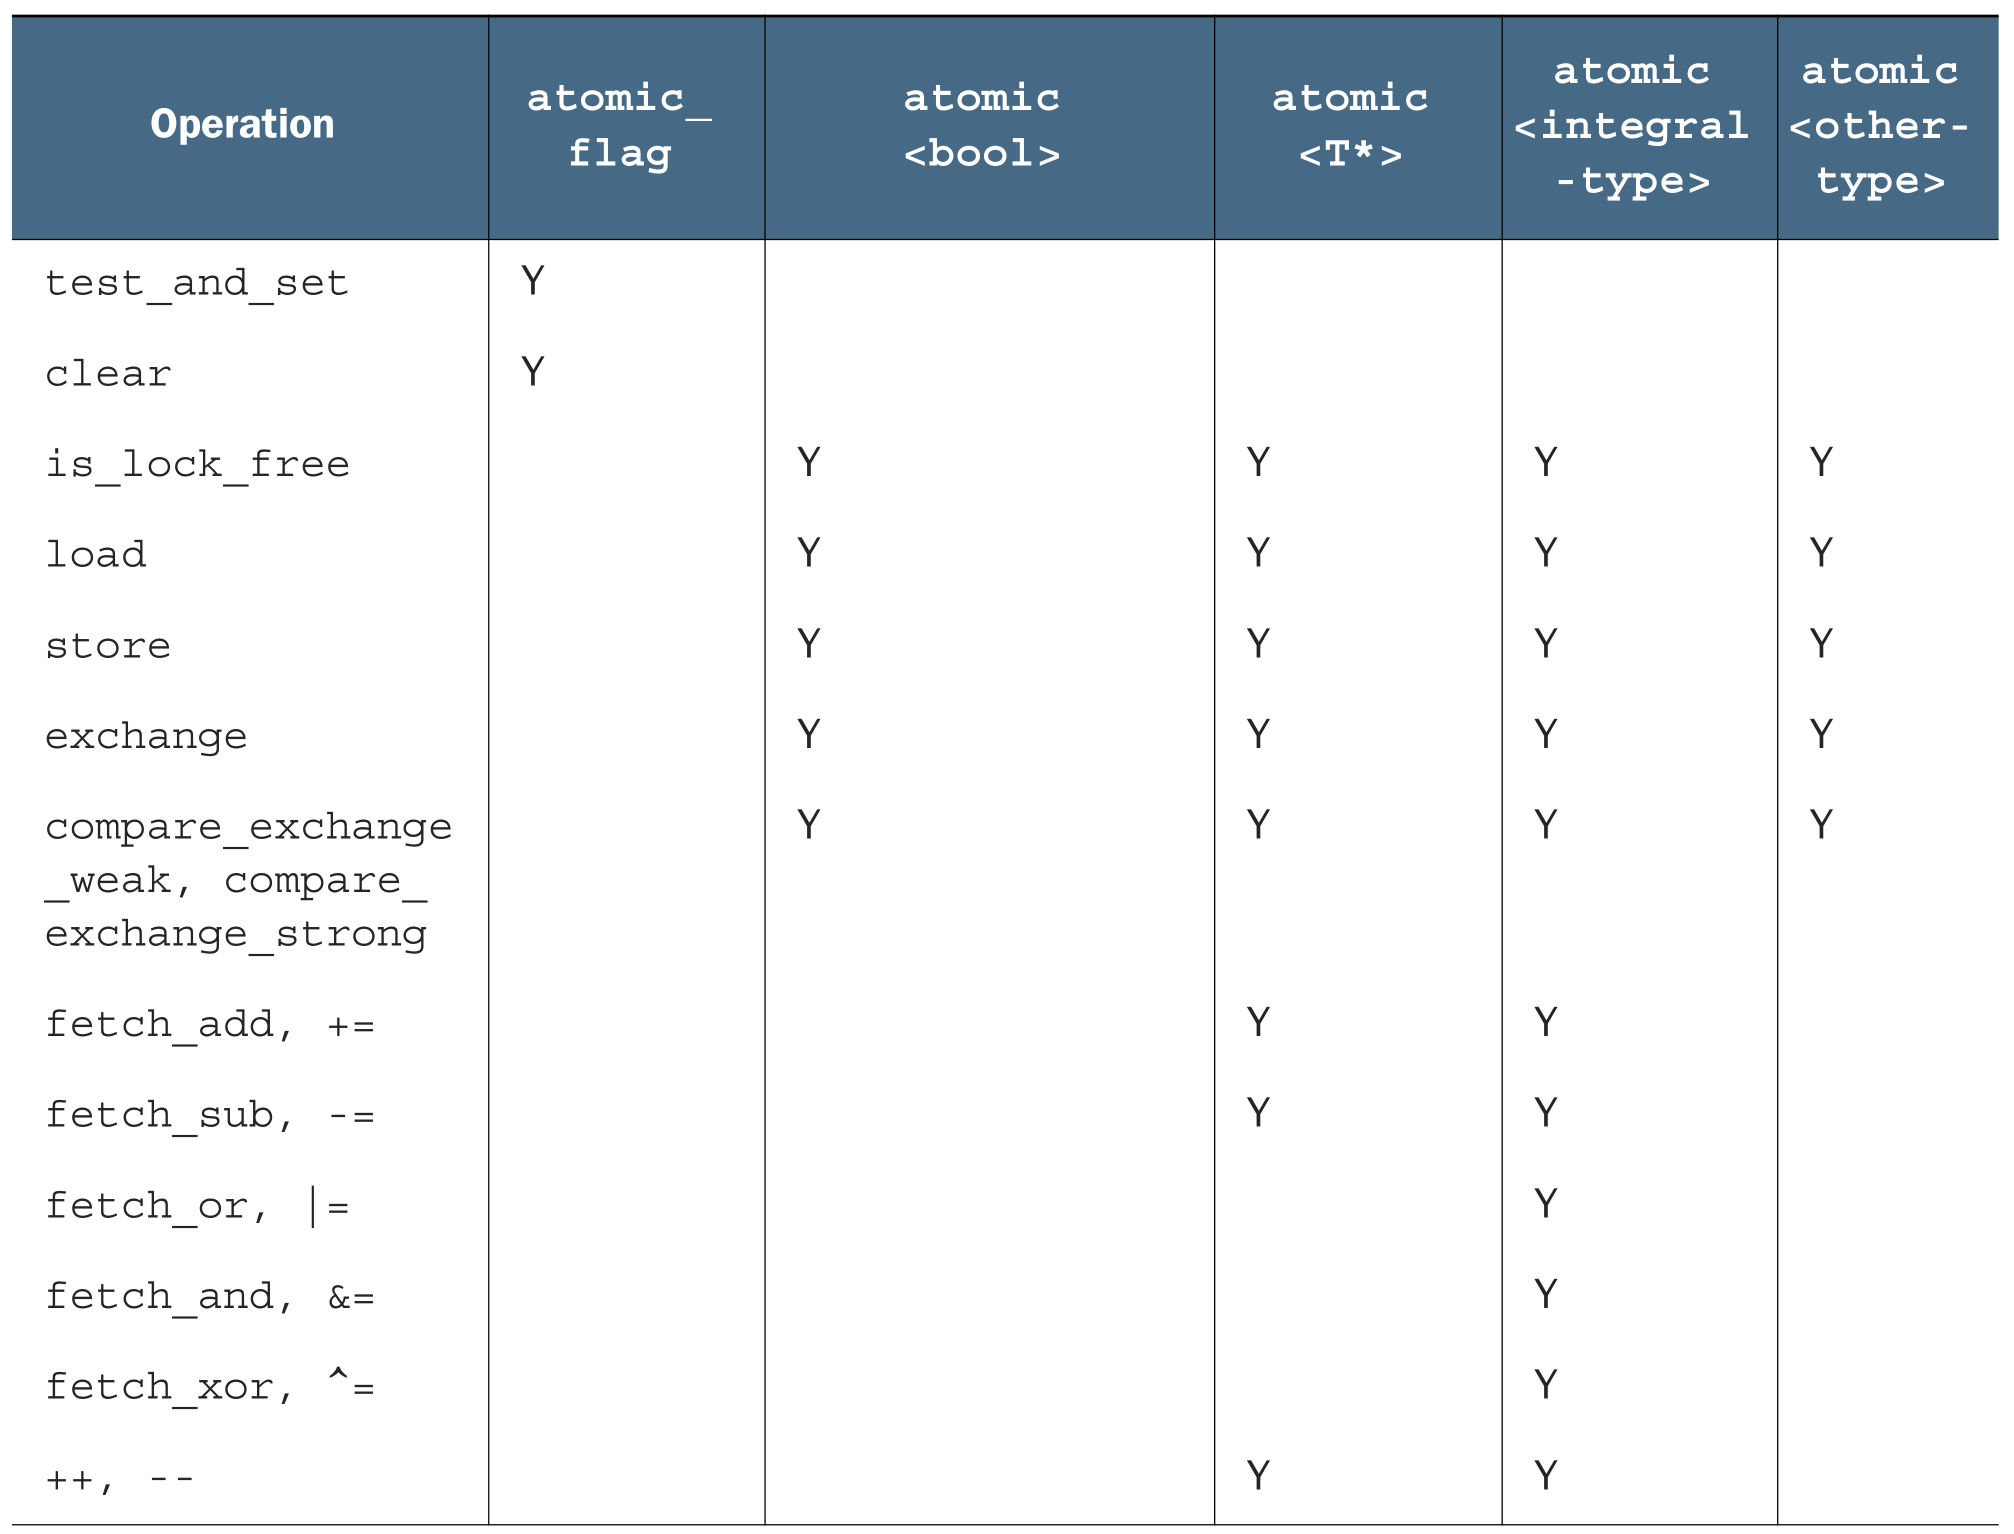
\includegraphics[width=0.7\textwidth]{content/chapter05/images/5-3-table.png}\\
    表5.3 每一个原子类型所能使用的操作
\end{center}

\mySubsubsection{5.2.7}{原子操作的非成员函数}

直到现在,还没有去描述成员函数对原子类型操作的形式,不同的原子类型中也有等价的非成员函数存在。大多数非成员函数的命名与对应成员函数有关,需要\texttt{atomic\_}作为前缀(比如,\texttt{std::atomic\_load()})。这些函数都会重载不同的原子类型,指定内存序时会分成两种:一种没有标签,另一种以\texttt{\_explicit}为后缀,并且需要额外的参数,或将内存序作为标签,亦或只有标签(例如,\texttt{std::atomic\_store(\&atomic\_var,new\_value)}与\texttt{std::atomic\_store\_explicit(\&atomic\_var,new\_value,std::memory\_order\_release)})。不过,成员函数隐式引用原子对象,所有非成员函数都持有一个指向原子对象的指针(作为第一个参数)。

例如,\texttt{std::atomic\_is\_lock\_free()}只有一种类型(虽然会被其他类型所重载),并且对于同一个对象a,\texttt{std::atomic\_is\_lock\_free(\&a)}返回值与a.is\_lock\_free()相同。同样的,\texttt{std::atomic\_load(\&a)}和a.load()的作用一样。需要注意的是,\texttt{a.load(std::memory\_order\_acquire)}与\texttt{std::atomic\_load\_explicit(\&a, std::memory\_order\_acquire)}的操作相同。

非成员函数的设计是为了与C语言兼容,C语言中没有引用。例如,compare\_exchange\_weak()和compare\_exchange\_strong()成员函数的第一个参数(期望值)是一个引用,而\texttt{std::atomic\_compare\_exchange\_weak()}(第一个参数是指向对象的指针)的第二个参数是一个指针。\texttt{std::atomic\_compare\_exchange\_weak\_explicit()}也需要指定成功和失败的内存序,而“比较/交换”成员函数都有一个单内存序(默认是\texttt{std::memory\_order\_seq\_cst}),重载函数可以分别获取成功和失败内存序。

对\texttt{std::atomic\_flag}的操作是“反潮流”的,那些操作中它们“标志”的名称为:\texttt{std::atomic\_flag\_test\_and\_set()}和\texttt{std::atomic\_flag\_clear()},但是以\texttt{\_explicit}为后缀的额外操作也能够指定内存顺序:\texttt{std::atomic\_flag\_test\_and\_set\_explicit()}和\texttt{std::atomic\_flag\_clear\_explicit()}。

C++标准库也对原子类型中的\texttt{std::shared\_ptr<>}智能指针类型提供非成员函数,这打破了“只有原子类型,才能提供原子操作”的原则。\texttt{std::shared\_ptr<>}不是原子类型,但是C++标准委员会认为这很重要。可使用的原子操作有:load, store, exchange和compare/exchange,这些操作重载了标准原子类型的操作,并且可获取\texttt{std::shared\_ptr<>*}作为第一个参数:

\begin{cpp}
std::shared_ptr<my_data> p;
void process_global_data()
{
  std::shared_ptr<my_data> local=std::atomic_load(&p);
  process_data(local);
}
void update_global_data()
{
  std::shared_ptr<my_data> local(new my_data);
  std::atomic_store(&p,local);
}
\end{cpp}

作为和原子操作一同使用的其他类型,也提供\texttt{\_explicit}变量,允许指定所需的内存序,并且\texttt{std::atomic\_is\_lock\_free()}函数可以用来确定实现是否使用锁,来保证原子性。

并行技术规范扩展提供了一种原子类型\texttt{std::experimental::atomic\_shared\_ptr<T>},该类型声明在\texttt{<experimental/atomic>}头文件中。和\texttt{std::atomic<UDT>}一样,也有load,store,exchange,compare-exchange这些操作。这个类型支持无锁实现,所以可以作为独立类型提供,并不会给普通的\texttt{std::shared\_ptr}实例增加开销。不过和\texttt{std::atomic}模板一样,可以使用成员函数is\_lock\_free,可以确定在对应的硬件平台上检查是否无锁。当实现不是无锁结构时,推荐使用\texttt{std::experimental::atomic\_shared\_ptr}原子函数,因为该类型会让代码更加清晰,确保所有的访问都是原子的,并且能避免由于忘记使用原子函数导致的数据竞争。与原子类型和操作一样,如想用原子操作对应用进行加速,就需要对其性能进行分析,并且与其他同步机制进行对比。

如之前的描述,标准原子类型不仅仅是为了避免数据竞争所造成的未定义行为,还允许用户对不同线程上的操作进行强制排序。这种强制排序是数据保护和同步操作的基础,例如:\texttt{std::mutex}和\texttt{std::future}。

所以,本节展示了内存模型在并发方面的细节,接下来回来介绍如何使用原子操作同步数据和强制排序。